%!TEX program = xelatex
\documentclass{beamer}

\usepackage{blindtext}
\usepackage[absolute,overlay]{textpos}
\usepackage{graphicx} % for pdf, bitmapped graphics files
\graphicspath{ {gm22may2018/images/} }

\usetheme{Execushares}
\def\checkmark{\tikz\fill[scale=0.4](0,.35) -- (.25,0) -- (1,.7) -- (.25,.15) -- cycle;}

\title{Back-Pressure based NoC to provide guaranteed and In-Order packet deliveries}
\subtitle{An overall review of how things stand right now}
\author{Gurshaant Malik}
\date{\today}

\setcounter{showSlideNumbers}{1}

\begin{document}
	\frame{\titlepage}
	\begin{frame}
		\frametitle{What are the 4 designs?}
		\pause
		\begin{enumerate}
			\item The back-pressure based design.
			\pause
			\item The local deflection based design.
			\pause 
			\item CMU CONNECT.
			\pause
			\item AXI-4 Stream Interconnect.\pause(A Xilinx IP).
		\end{enumerate}
	\end{frame}

	\setcounter{showProgressBar}{1}
	\setcounter{showSlideNumbers}{1}
	
	\section{CMU Connect}
	
	    \begin{frame}\frametitle{Specifications}
	    \begin{textblock*}{3.5cm}(3.5cm, 2.5cm) % {block width} (coords)
	        \visible<1>{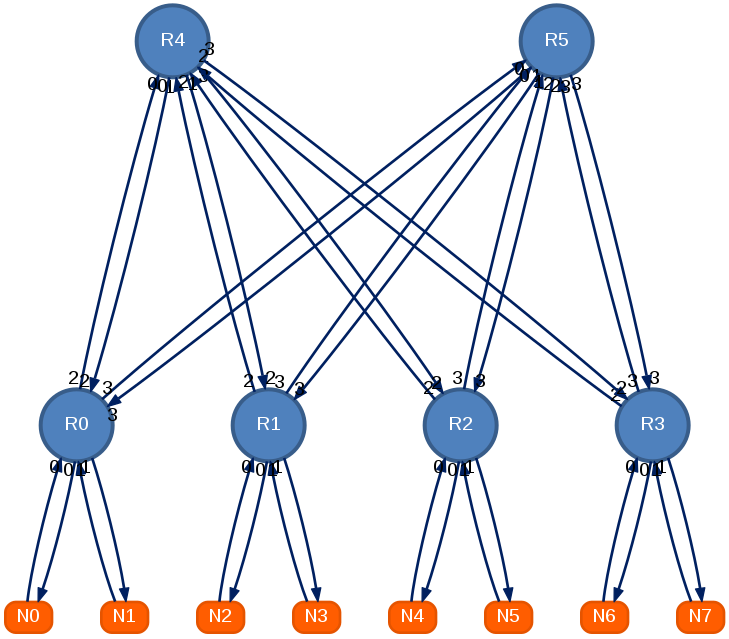
\includegraphics[scale=0.25]{cmu_connect.png}}
	    \end{textblock*}
	    \pause
	    \begin{itemize}
	        \item Simple Input Queued.
	        \pause
	        \begin{itemize}
	            \item Flit buffer depth = 8.
	        \end{itemize}
	        \pause
	        \item Peak Flow Control
	        \pause
	        \begin{itemize}
	            \item No Virtual Links.
	        \end{itemize}
	        \pause
	        \item Separate Input-First Round-Robin allocator.
	    \end{itemize}
	    \pause
	    \begin{textblock*}{3cm}(9cm, 5.5cm) % {block width} (coords)
            \visible<2,3,4,5,6>{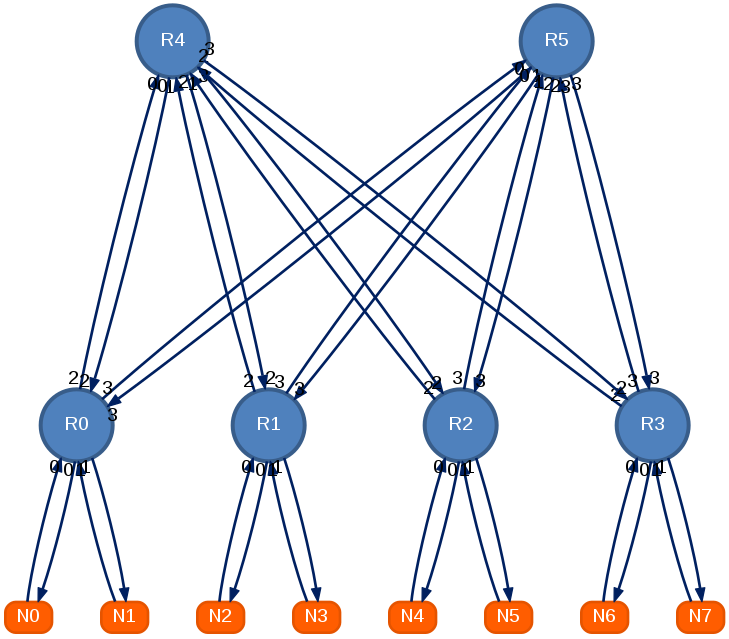
\includegraphics[height=3.5cm, width=3.5cm]{cmu_connect.png}}
        \end{textblock*}
	    \end{frame}
	    
	    \begin{frame}\frametitle{Advantages}
	    \pause
	    \begin{itemize}
	        \item Provide In-Order delivery.
	        \pause
	        \item Guaranteed packet delivery.
	        \pause
	        \item High throughput.
        \end{itemize}
	    \end{frame}
	    
	    \begin{frame}\frametitle{Disadvantages}
	    \pause
	    \begin{itemize}
	        \item Bloated design. High area consumption.
	        \pause
	        \item Slow peak frequency.
	        \pause
	        \item Not scalable. Supports maximum of 64 clients.
        \end{itemize}
	    \end{frame}
	    
	\section{Local Deflection NoC}
	    \begin{frame}{Specifications}
	    \pause
	    \visible<2,3>{\begin{itemize}
	        \item Buffer-Less design.
	        \pause
	        \item Local deflections to manage contention.
	    \end{itemize}}
	    
	    {\begin{textblock*}{3.5cm}(3cm, 3.5cm) % {block width} (coords)
	        \visible<4>{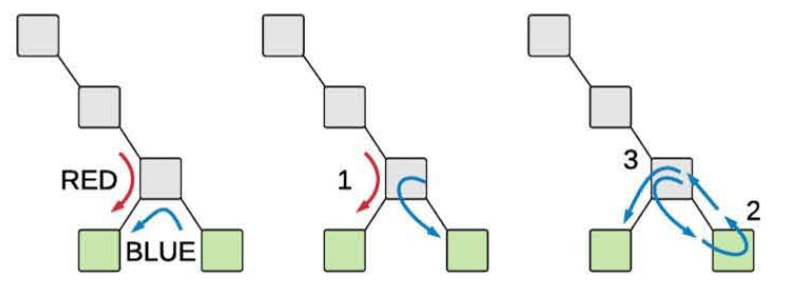
\includegraphics[scale=0.25]{local.png}}
	    \end{textblock*}}
	    \end{frame}
	    
	    \begin{frame}\frametitle{Advantages}
	    \pause
	    \begin{itemize}
	        \item FPGA resource efficient.
	        \pause
	        \item Meets high frequency targets.
	        \pause
	        \item High throughput.
	        \pause
	        \item Scalable to support increasing number of clients.
        \end{itemize}
	    \end{frame}	    
	    
	    \begin{frame}\frametitle{Disadvantages}
	    \pause
	    \begin{itemize}
	        \item No guarantee of packet delivery.
	        \pause
	        \item Packets do not get delivered in-order.
        \end{itemize}
	    \end{frame}		  
	    
	\section{AXI4 Stream Interconnect}
	    \begin{frame}{Specifications}
	    \pause
	    \begin{itemize}
	        \item One highly optimized cross-bar switch.
	        \pause
	        \item Round-Robin/Fixed Priority arbiter.
	        \pause
	        \item AXI-4-Stream interface.
	    \end{itemize}
	    \end{frame}
	    
	    \begin{frame}\frametitle{Advantages}
	    \pause
	    \begin{itemize}
	        \item Highly optimized resource consumption.
	        \pause
	        \item Meets high frequency targets.
	        \pause
	        \item In-Order packet delivery.
	        \pause
	        \item Plug-and-Play HLS/Proprietary-RTL IPs.
        \end{itemize}
	    \end{frame}	
	    
	    \begin{frame}\frametitle{Disadvantages}
	    \pause
	    \begin{itemize}
	        \item Not scalable. Supports at maximum 16 clients.
	        \pause
	        \item Tightly tied to Xilinx FPGAs.
	        \pause
	        \item High queuing times.
	        \pause
	        \item Fixed priority arbitration will not provide guaranteed delivery.
        \end{itemize}
	    \end{frame}	
	
	\section{The Back-Pressure NoC}
        \begin{frame}
        \frametitle{What are the design wins?}
           \pause
           It is the only design that achieves all of the following:
           \pause
           \begin{itemize}
               \item Guaranteed packet delivery.
               \pause 
               \item In-Order packet delivery.
               \pause
               \item Scales to support any number of clients.
               \pause
               \item FPGA resource efficient.
               \pause
               \item Meets frequency targets of 300MHz+
               \pause
               \item AXI-4-Stream Compatible.
           \end{itemize}
        \end{frame}
        
        \begin{frame}{Specifications:}
        \pause
            \visible<2,3,4,5,6,8,9>{\begin{itemize}
                \item Round Robin. Ensures packet progress.
                \begin{itemize}
                    \pause
                    \item Fair.
                    \pause
                    \item Smart.
                \end{itemize}
                \pause
                \item Quantified up-stream paths. Ensures In-Order.
                \pause
                \begin{itemize}
                    \item Concrete path for each src-dest pair.
                \end{itemize}
                \pause
                \pause
                \item Back-Pressure. Ensures In-Order.
                \pause
                \begin{itemize}
                    \item Younger flit cannot overtake older flit.
                \end{itemize}
            \end{itemize}}
            {\begin{textblock*}{3.5cm}(3cm, 2.5cm) % {block width} (coords)
	            \visible<7>{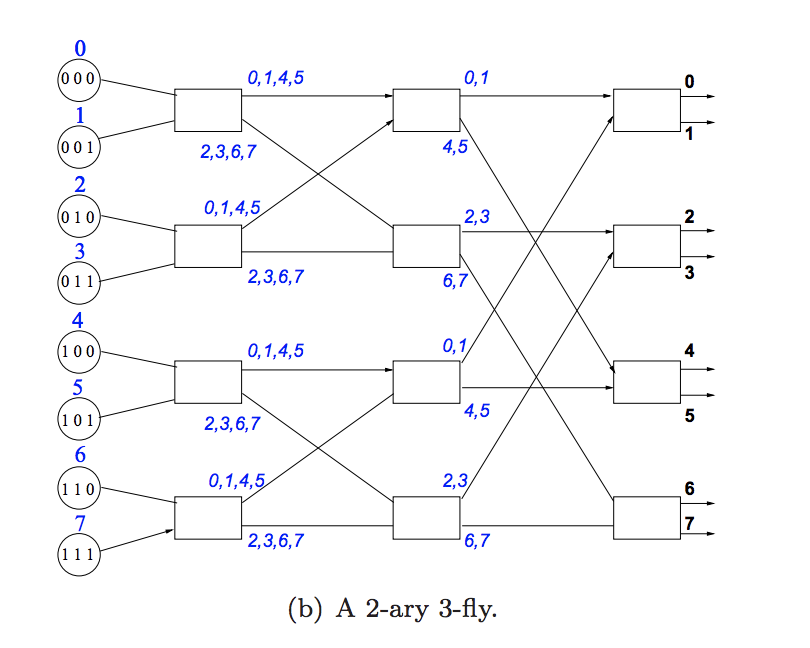
\includegraphics[scale=0.5,trim={0 1cm 0 0},clip]{inorder.png}}
	        \end{textblock*}}
	        {\begin{textblock*}{3.5cm}(3cm, 3.5cm) % {block width} (coords)
	            \visible<10>{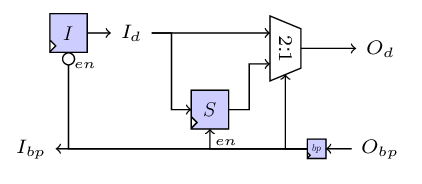
\includegraphics[scale=0.5]{28.png}}
	        \end{textblock*}}
        \end{frame}
        
        \begin{frame}{Disadvantages}
            \pause
            \begin{itemize}
                \item Slightly reduced throughput owing to limitation of upstream climbing.
                \pause
                \item Slower frequency and bloated area compared to Local Deflection and Xilinx's Interconnect.
                \pause
                \begin{itemize}
                    \item Still 300MHz+.
                    \pause
                    \item Still $\leq$ 500 LUTS at maximum.
                \end{itemize}
            \end{itemize}
        \end{frame}
        
        \section{Comparison Overview}
        \begin{frame}{Feature Checklist}
            \begin{center}
                \begin{tabular}{c c c c c} 
                    \hline
                    & \textbf{CMU} & \textbf{LD} & \textbf{AXI-IC} & \textbf{BP} \\ [0.5ex] 
                    \hline\hline
                    \pause
                    \textbf{Guaranteed Delivery} & \checkmark & X & \checkmark & \checkmark \\ 
                    \hline
                    \pause
                    \textbf{In-Order Delivery} & \checkmark & X & \checkmark & \checkmark \\ 
                    \hline
                    \pause
                    \textbf{Scalable} & X & \checkmark & X & \checkmark \\ 
                    \hline
                    \pause
                    \textbf{Frequency Targets} & X & \checkmark & \checkmark & \checkmark \\  
                    \hline
                    \pause
                     \textbf{AXI4-S Compatible} & X & X & \checkmark & \checkmark \\  
                    \hline
                \end{tabular}
            \end{center}
        \end{frame}
        
        \begin{frame}{Test Environment Overview}
        \begin{itemize}
            \item Data Width : 32 bits
            \pause
            \item Real and Synthetic communication patterns
            \pause
            \item Number of Clients varied from N=2 to 128, in powers of 2.
            \pause
            \item Injection rate varied from 1 to 100.
            \pause
            \item Topologies : TREE, XBAR, MESH0, MESH1.
        \end{itemize}
        \end{frame}
        
        \begin{frame}{Metrics}
        \begin{itemize}
            \item Sustained Throughput.
            \pause
            \item Worst queuing latency.
            \pause
            \item Worst in-flight latency.
            \pause
            \item Area of the NoC.
            \pause
            \item Frequency of the NoC.
        \end{itemize}
        \end{frame}
        
        \begin{frame}{BP vs LD : TREE}
        \pause
      	{\begin{textblock*}{3.5cm}(-0.8cm, 1cm) % {block width} (coords)
	        \visible<2>{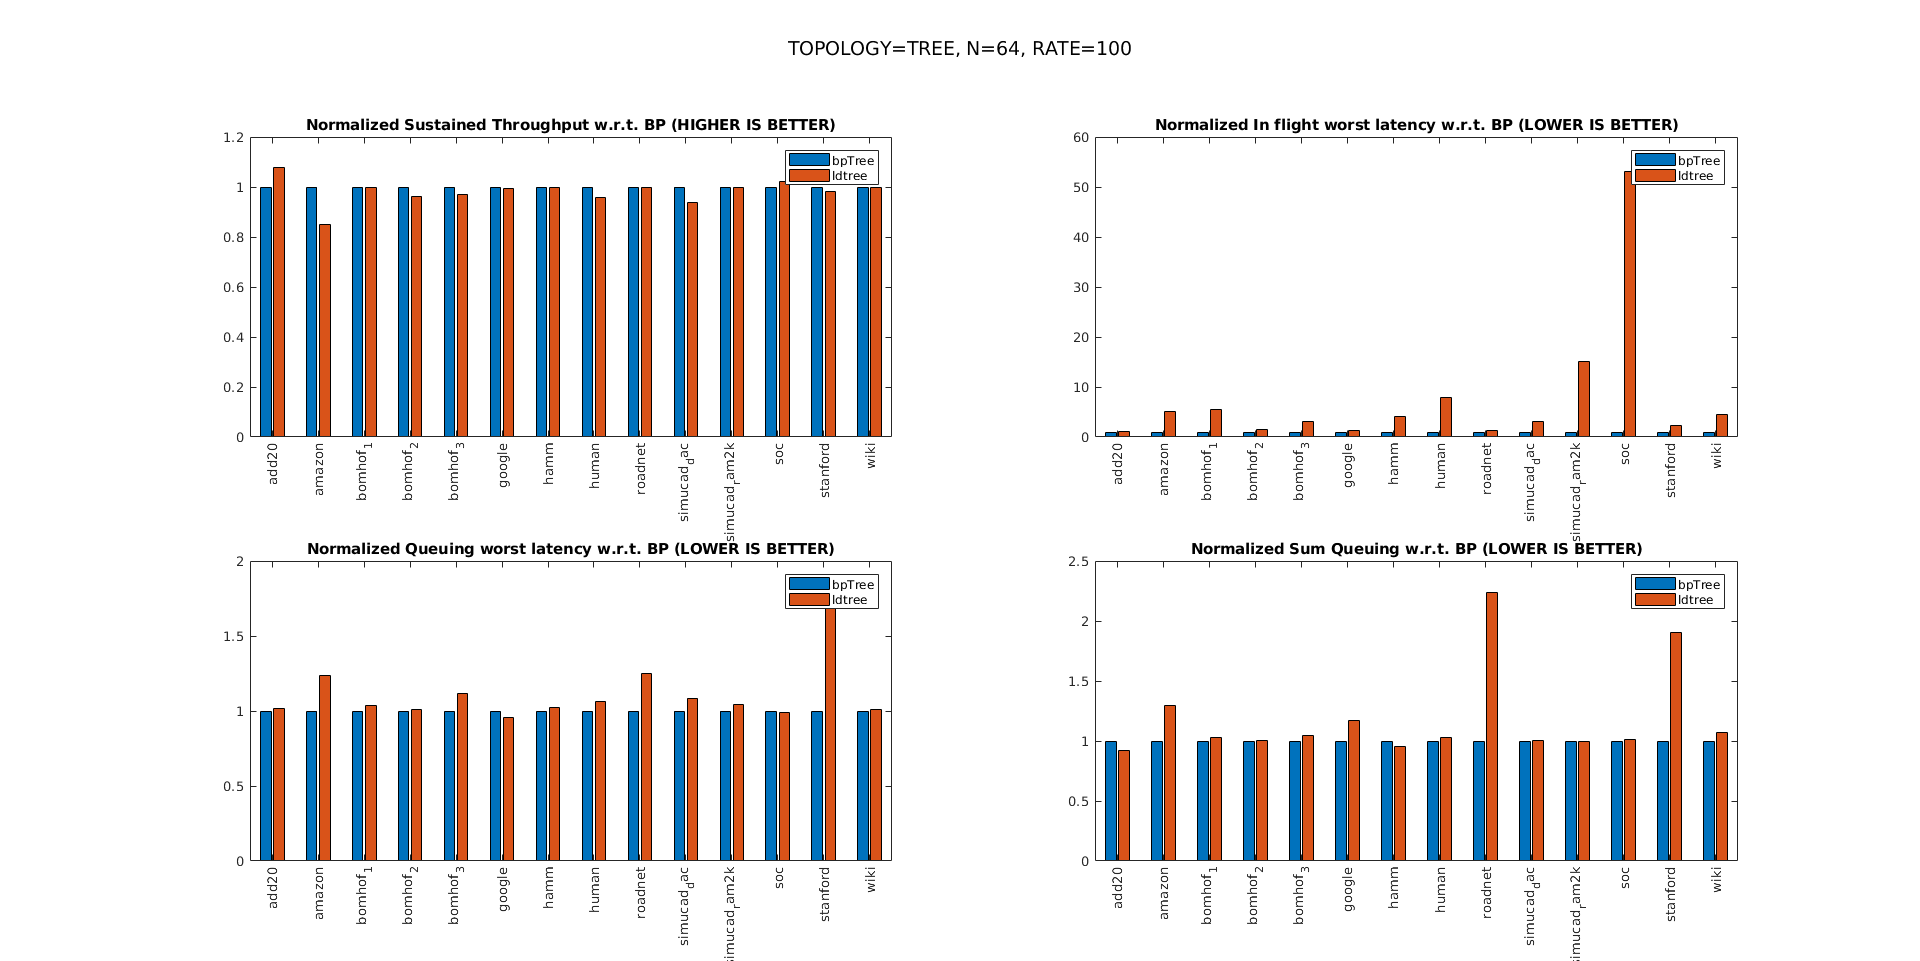
\includegraphics[width=14cm,height=8cm]{tree_n64_r100.png}}
	    \end{textblock*}}
        \end{frame}
        
        \begin{frame}{BP vs LD : MESH0}
        \pause
      	{\begin{textblock*}{3.5cm}(-0.8cm, 1cm) % {block width} (coords)
	        \visible<2>{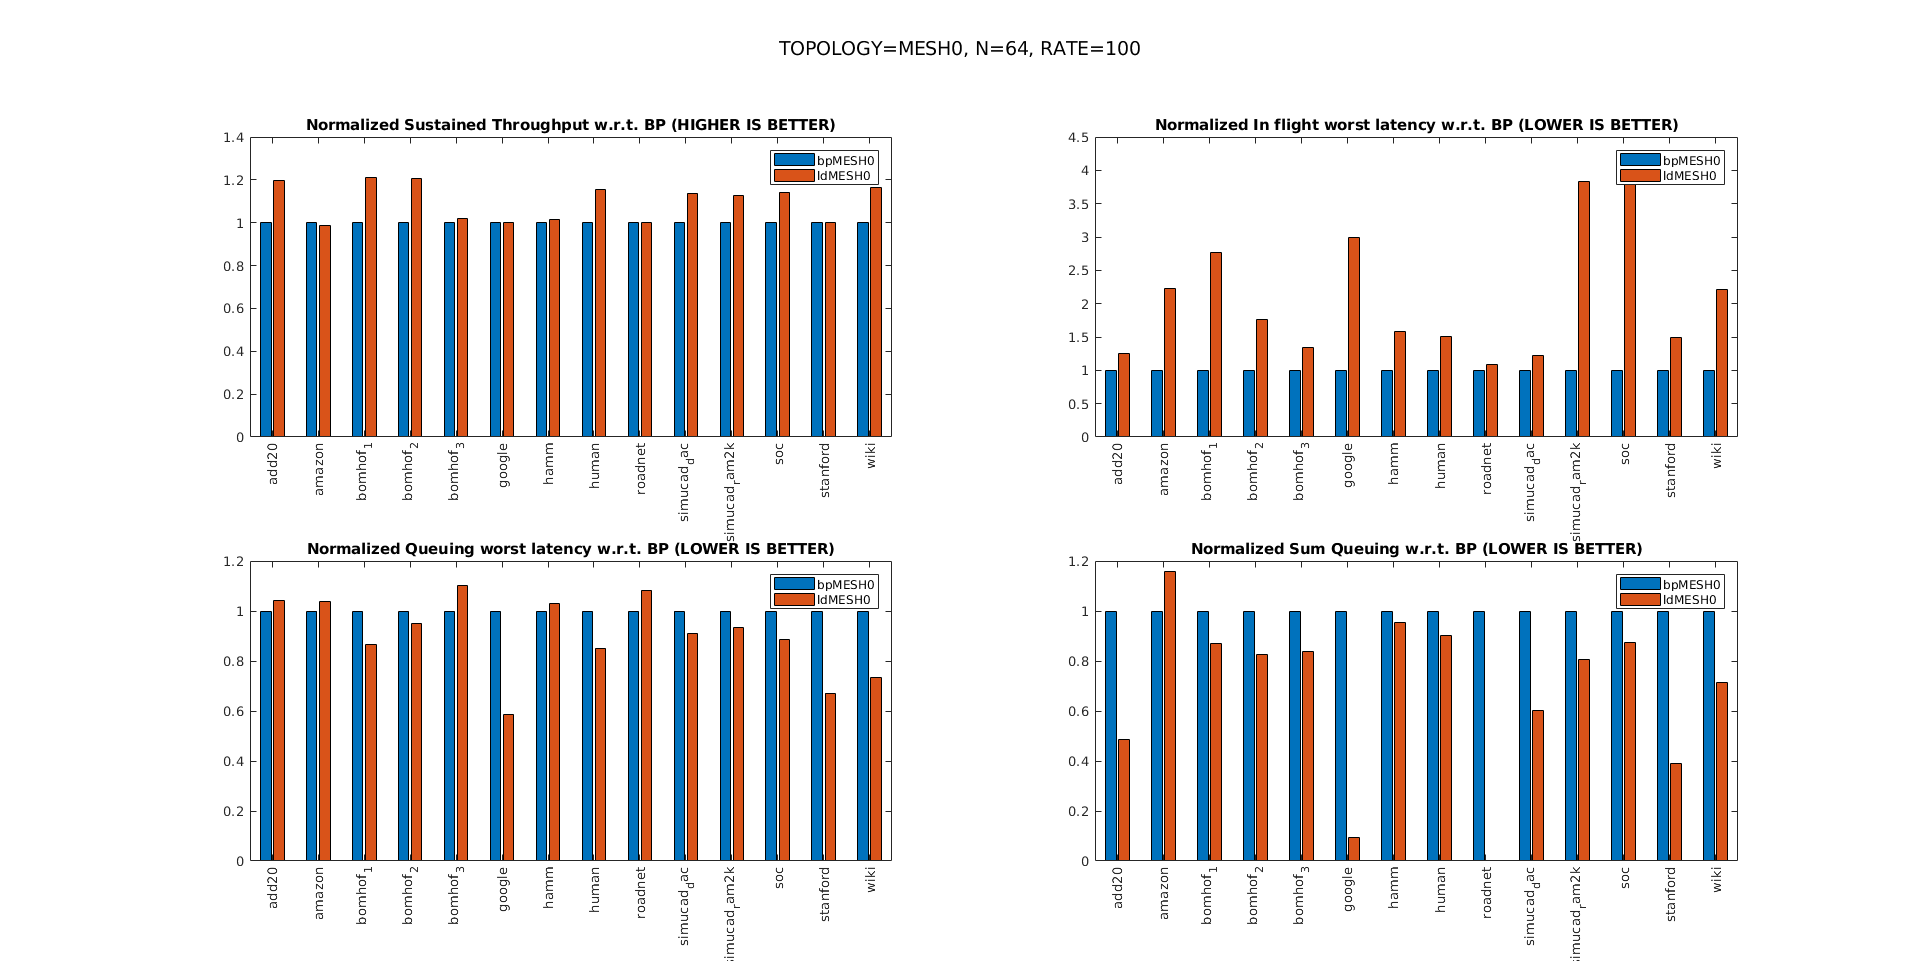
\includegraphics[width=14cm,height=8cm]{mesh0_n64_r100.png}}
	    \end{textblock*}}
        \end{frame}
        
        \begin{frame}{BP vs LD : MESH1}
        \pause
      	{\begin{textblock*}{3.5cm}(-0.8cm, 1cm) % {block width} (coords)
	        \visible<2>{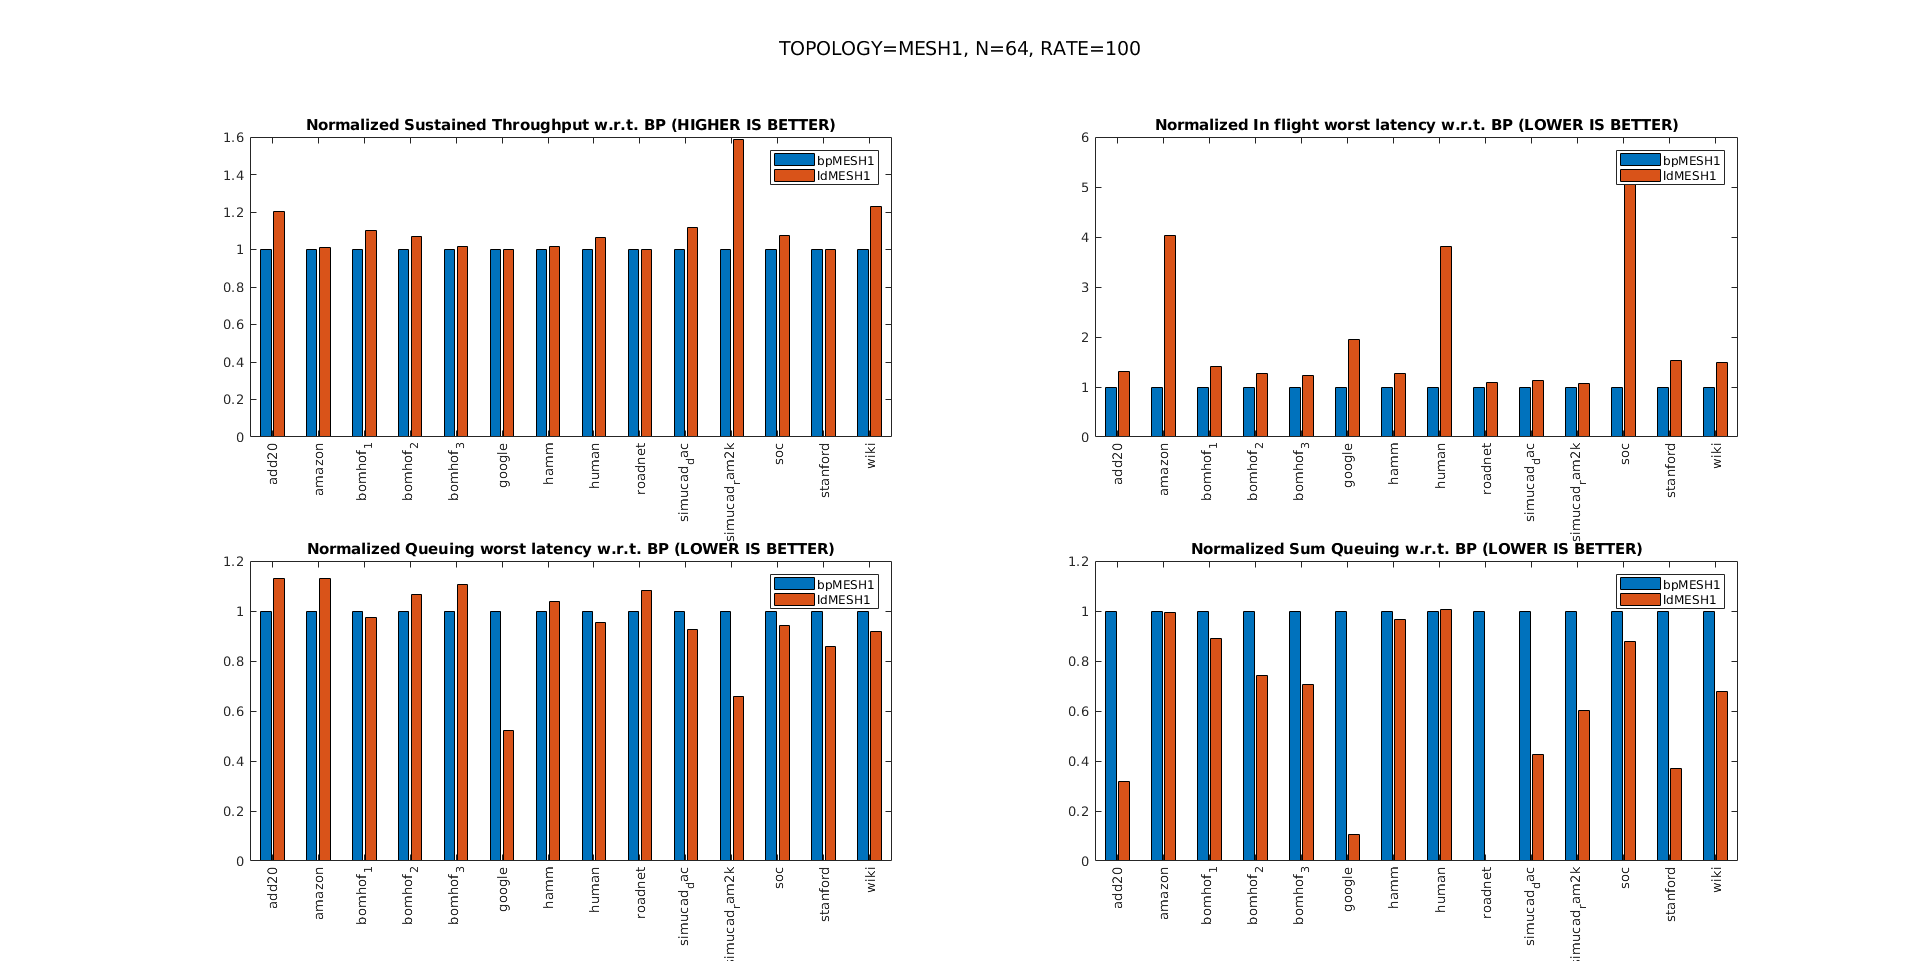
\includegraphics[width=14cm,height=8cm]{mesh1_n64_r100.png}}
	    \end{textblock*}}
        \end{frame}

        \begin{frame}{BP vs LD : XBAR}
        \pause
      	{\begin{textblock*}{3.5cm}(-0.8cm, 1cm) % {block width} (coords)
	        \visible<2>{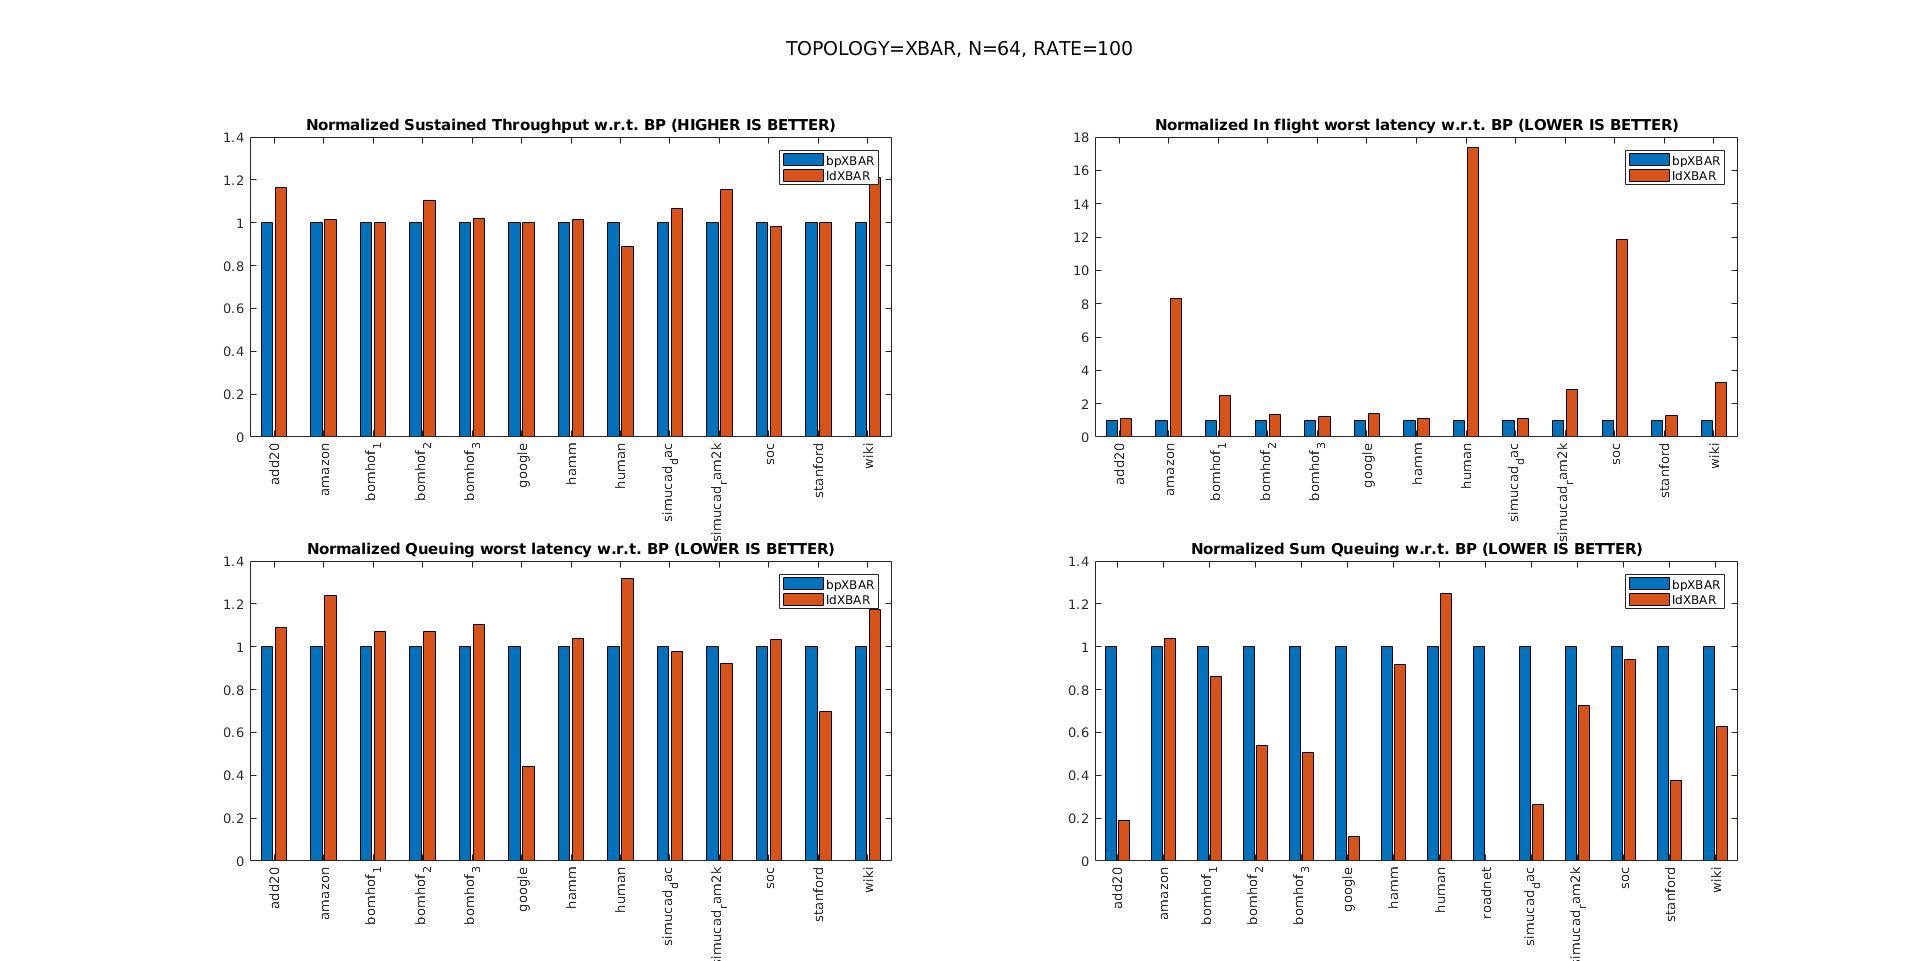
\includegraphics[width=14cm,height=8cm]{xbar_n64_r100.png}}
	    \end{textblock*}}
        \end{frame}  
        
       \begin{frame}{Frequency and Area(N=16, Virtex 7)}
            \begin{center}
                \resizebox{\columnwidth}{!}{%
                \begin{tabular}{c c c c c c c} 
                    \hline
                    & \textbf{CMU} & \textbf{LD(TREE)} & \textbf{LD(XBAR)} & \textbf{AXI-IC} & \textbf{BP(TREE)} & \textbf{BP(TREE)}\\ [0.5ex] 
                    \hline\hline
                    \pause
                    \textbf{Peak Frequency(MHz)} & ?100? & 597 & 430 & 400 & 440 & 350\\ 
                    \hline
                    \pause
                    \textbf{Area(LUTS)} & ?  & 2115 &  7000 & 6893 & 16000 & 3285\\ 
                    \hline
                \end{tabular}}
            \end{center}
            \pause
            \begin{itemize}
                \item These numbers can get even better.
            \end{itemize}
        \end{frame} 
        
        \begin{frame}{Summary}
        \pause
                \begin{center}
                \begin{tabular}{c c c c c} 
                    \hline
                    & \textbf{CMU} & \textbf{LD} & \textbf{AXI-IC} & \textbf{BP} \\ [0.5ex] 
                    \hline\hline
                    \textbf{Guaranteed Delivery} & \checkmark & X & \checkmark & \checkmark \\ 
                    \hline
                    \textbf{In-Order Delivery} & \checkmark & X & \checkmark & \checkmark \\ 
                    \hline
                    \textbf{Scalable} & X & \checkmark & X & \checkmark \\ 
                    \hline
                    \textbf{Frequency Targets} & X & \checkmark & \checkmark & \checkmark \\  
                    \hline
                     \textbf{AXI4-S Compatible} & X & X & \checkmark & \checkmark \\  
                    \hline
                \end{tabular}
            \end{center}
            \begin{itemize}
            \pause
                \item Throughput : Neck to Neck vs LD.
                \pause 
                \item InFlight latency : 4x to 10x better vs LD.
                \pause
                \item Queuing : Neck to Neck vs LD. Few Exceptions.
            \end{itemize}
        \end{frame} 
        
        \begin{frame}{Remaining Tasks}
        \pause
            \begin{itemize}
                \item Analyze results of CMU Connect.
                \pause 
                \item Optimize frequency and area numbers on XVU9P FPGA.
                \pause
                \item Write the paper.
            \end{itemize}
        \end{frame} 
        




\end{document}
